\cut{
1. (way ahead of time) train a statistical model over the training data
2. (at inference time) coarse-grain tokenization (i.e. finding Seqsets)
3a. run the statistical model over the user data, and use the (modified) 
    viterbi algorithm to find the most likely sequences
3b. populate histograms based on the most likely sequences
3c. select candidate histograms + structure, according to heuristics
3d. break down Seqsets using not just the most likely sequences
3e. recursively repeat, go to 3a.
4. apply rewriting involving blob finding to maximize the information 
   theoretic complexity score

We'll compose this algorithm by figure and explain it with running examples 
in Section 2.
}

\section{The Format Inference Algorithm}\label{sec:algo}

Our new format inference algorithm consists of four stages:
(1) building a statistical token model from labeled training data;
(2) dividing the text into newline-separated {\em chunks} of data 
and finding all possible tokenizations of each chunk; (3)
inferring a {\em candidate structure} using the statistical model
and the tokenizations; and (4) applying rewriting rules to improve 
the candidate structure.
%\end{enumerate}
Because this algorithm shares the general structure of
our earlier work~\cite{fisher+:dirttoshovels}, we focus on the 
salient differences here.


% The basic approach is to break the
% input into units of repetition, called {\em chunks}, and then to
% analyze these chunks for patterns that reveal the structure
% of the data.  Depending upon the data source, the unit of repetition
% might be a file, a collection of lines within a file that constitute
% some notion of ``paragraph,'' a new-line terminated line, characters
% terminated by pipes, \etc{}

% The algorithm includes four main phases:
% {\em training the statistical model}, 
% {\em probablistically tokenizing} the raw data, 
% performing recursive {\em structure discovery},
% and using rewriting rules to do {\em format refinement}. 
% This algorithm is similar to the one proposed in our earlier work
% \cite{fisher+:dirttoshovels}.  
% The new algorithm differs in that it defers decisions about
% tokenization until structure discovery. 
% In particular, the tokenization phase produces the set of {\em all
% possible} token sequences for each data chunk in a data structure
% called a \seqset{}.  The structure
% discovery phase then incrementally selects the appropriate sequence from
% the \seqset{} as it builds a description of the data.


% %(3a) find the most probable token sequence for each chunk, and 
% %     if that sequence of every chunk contains only 1 or 0 edges 
% %     then return else go to (3b)
% %(3b) construct histograms from the most probably sequences and 
% %     predict a top-level structure;
% %(3c) populate sub-components of the predicated structure with \seqset's
% %     or sub-\seqset's;
% %(3d) for each sub-component, recurse to (3a);

% % \begin{figure}[t]
% % \begin{centercode}
% % (1) Train a statistical model from labeled training data
% % (2) Tokenize raw data into \seqset{}s, one \seqset{} per chunk
% % (3) Discover initial structure using the \seqset{}s
% % (4) Apply rewriting rules to improve the overall structure
% % \end{centercode}
% % \caption{High-level Inference Algorithm}\label{fig:algo}
% % \end{figure}

% \figref{fig:algo} summarizes the high-level algorithm.  In the
% following sections, we explain the pieces in more detail using the
% \texttt{yum.txt} format as a running example.
% Because this algorithm shares the general structure of
% the original algorithm, we only highlight the differences here, 
% refering the reader to the earlier paper~\cite{fisher+:dirttoshovels}
% for complete discussion of the original algorithm.

\paragraph*{Training the statistical models.}

% Before attempting to discover the structure of any particular format,
% we train a statistical model to tokenize ad hoc data using a large
% pool of sample data formats.  Intuitively, we can then use the
% resulting model to infer formats for any ad hoc data source that uses
% the tokens found in the training data.  Hence, we only need to
% rerun this phase of the algorithm when given ad hoc data with
% fundamentally different kinds of tokens.  

To speed up the training cycle, we created a tool
capable of reading any \pads{} description and labelling the
described data with the tokens specified in the description.  This way,
all data for which we have \pads{} descriptions can serve as a training
suite. As we add more descriptions, our training data
improves.  Currently, the training suite is biased towards systems 
data, and includes
tokens for integers, floats, times, dates, IP addresses, hostnames, 
file paths, URLs, words, ids and punctuation. 
%A given substring may be parsed by more than one of the token
%types, and we pick a token that best represent the meaning of the data.
Parsing of tokens continues to use longest match semantics
and hence the string ``43.8'' can be parsed by sequences such as
{\tt [int] [.] [int]} or {\tt [int] [.] [float]} or {\tt [float]},
but not by {\tt [float] [.] [int]} or {\tt [float] [.] [float]}.
%because the token {\tt float} would parse the entire string, even though
%the string ``43'' alone can be represented by a {\tt [float]}.
We have experimented with a number of statistical models for
tokenization, which we discuss in \secref{sec:stats}.

\paragraph*{Tokenization.}

When inferring a description, the algorithm computes the set of all
possible tokenizations of each data chunk.  Because these sequences
share subsequences, we organize them into a directed acyclic graph
called a \seqset{}.  For example, \figref{fig:seqset} shows the \seqset{} for the substring 
``2.2.13-4''. 

%\figref{fig:seqset} shows the \seqset{} for the
%substring ``2.2.13-4'' from a chunk in \figref{fig:yum}. It forms a
%small part of the \seqset{} for the entire chunk.

\begin{figure}[th]
\begin{center}
\shrink
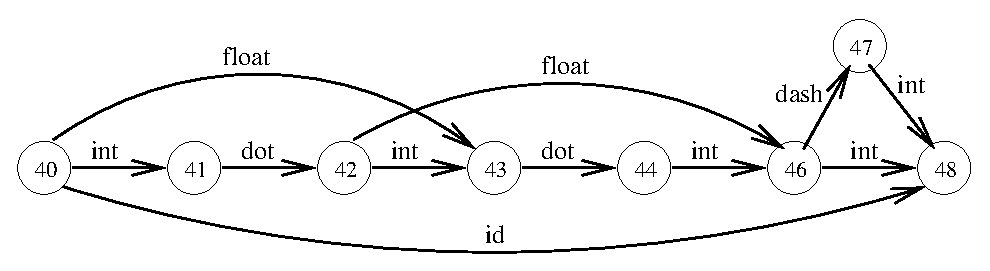
\epsfig{file=seqset.eps, width=0.7\columnwidth}
\end{center}
\caption{\seqset{} from parsing string ``2.2.13-4''.}\label{fig:seqset}
\shrink
\end{figure}

\noindent
Each edge in the \seqset{} represents an occurrence of a token in the
data, while each vertex marks a location in the input.  If a token
edge ends at a vertex $v$, then $v$ indicates the position immediately
after the last character in the token.  The first vertex in a
\seqset{} marks the position before the first character in its
outgoing edges. 
%The construction of the \seqset, though expensive, is done only once
%per token training session.  The algorithm subsequently uses the
%\seqset{} as input to the recursive structure discovery phase, which
%updates the \seqset{} during each recursive call.

\begin{figure}[t]
\begin{centercode}
type description  (* abstract syntax of pads description *)
type seqset       (* the seqset data structure *)
type seqsets = seqset list

(* A top-level description guess *)
datatype prophecy =
   BaseProphecy   of description
 | StructProphecy of seqsets list 
 | ArrayProphecy  of seqsets * seqsets * seqsets
 | UnionProphecy  of seqsets list

(* Guesses the best top-level description *)
fun oracle : seqsets -> prophecy

(* Implements a generic inference algorithm *)
fun discover (sqs:seqsets) : description =
 case (oracle sqs) of
   BaseProphecy b => b

 | StructProphecy sqss => 
     let Ts = map discover sqss in
     struct \{ Ts \}

 | ArrayProphecy (sqsfirst,sqsbody,sqslast) => 
     let Tfirst = discover sqsfirst in
     let Tbody  = discover sqsbody  in
     let Tlast  = discover sqslast  in
     struct \{ Tfirst; array \{ Tbody \}; Tlast; \}

 | UnionProphecy sqss => 
     let Ts = map discover sqss in
     union \{ Ts \}
\end{centercode}
\caption{A generic structure-discovery algorithm in Pseudo-ML.} 
\label{fig:structure-discovery}
\end{figure}

\paragraph*{Structure discovery.}
The structure discovery phase uses a {\em top-down}, {\em
divide-and-conquer} algorithm outlined in 
\figref{fig:structure-discovery} in the pseudo-ML function
\cd{discover}.  Each invocation of \cd{discover}
calls the \cd{oracle} function to guess the structure of the data represented
by the current set of \seqset{}s.  The oracle can prophesy
either a {\em base type}, a {\em struct}, an {\em array} or a {\em union}.
The {\tt oracle} function also partitions the input \seqset{}s into
sets of sub-\seqset{}s, each of which corresponds to a component in
the guessed structure.  The \cd{discover} function then recursively 
constructs the structure of each set of sub-\seqset{}s.

How does the \cd{oracle} produce its prophecy?
First, it uses the trained statistical model to assign probabilities
to the edges in the input \seqset{}s.
Next, it computes for each \seqset{} the {\em most probable token
sequence} (MPTS) among all the possible paths 
using a modified {\em Viterbi} algorithm \cite{rabiner89:hmm},
which we discuss in \secref{sec:stats}.
Then, based on the statistics of the tokens in the MPTSs,
the oracle predicts the structure of the current collection of
\seqset{}s using the heuristics designed for our earlier
algorithm~\cite{fisher+:dirttoshovels}. 

As an example, consider applying the oracle to determine the top-level
structure of the first line in \texttt{yum.txt}.  It would predict the
following: 
\begin{centercode}
struct \{date;  ' '; time; ' '; word; ':'; ' '; id; TBD\}
\end{centercode}
\ie{}, a \cd{struct} containing nine sub-structures including \cd{TBD}, which is
a sub-structure whose form will be determined recursively.
At this point, the {\tt oracle} partitions
every \seqset{} in the input into nine parts, corresponding to
sub-structure boundaries,
\ie{}, at the vertices after tokens \cd{date}, \cd{space}, \cd{time},
\etc{}
During partitioning, the oracle removes \seqset{} edges that cross partition
boundaries because such edges are irrelevant for the next round
of structure discovery.
For example, if the oracle cuts after the first {\tt float} token in the \seqset{}
in \figref{fig:seqset}, then it removes the \cd{id}~edge and the \cd{float} edge between
vertices~42 and~46, creating the two new \seqset{}s in \figref{fig:cut}.
%
\begin{figure}[th]
\begin{center}
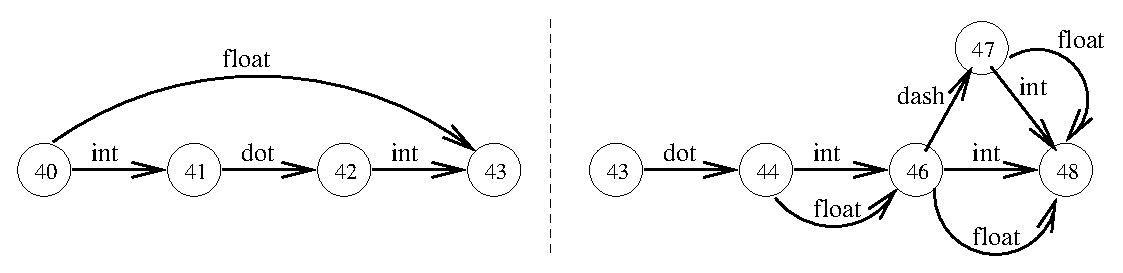
\epsfig{file=cut.eps, width=0.8\columnwidth}
\end{center}
\caption{Cutting \seqset{} for ``2.2.13-4'' after the first float token.} \label{fig:cut}
\shrink
\end{figure}
%
Finally, the {\tt oracle} function returns the predicted structure as a ``prophecy''
along with the partitioned \seqset{}s. 

\paragraph*{Format refinement with blob-finding.}
The refinement phase, which follows structure discovery, tries to
improve the initial rough structure by applying a series of
rewriting rules.  We have modified the earlier algorithm to use a 
``blob-finding'' rule.  This rule tries to identify data segments 
with highly complex, structured descriptions where none of the 
individual pieces of the description describe much of the data.
Intuitively, such occurrences correspond to places where the data
contained a high degree of variation, and the inference algorithm
built a description that enumerated all the possible variations in
painstaking detail. 
The blob rule replaces such complexity with a single \textit{blob} token.
A typical example of this kind
of data is free-form text comments that sometimes appear at the end of
each line in a log file.  The blob-finding rule reduces the overall
complexity of the resulting description and hence makes it more
readable.

The format refinement algorithm applies the blob-finding rule 
in a bottom-up fashion. It converts into a blob each sub-structure
that it deems overly complex and for which it can find a terminating pattern. 
The \pads{} parser uses the terminating pattern to
find the extent of the blob. The algorithm merges adjacent blobs.

To decide whether a given structure is a blob, 
the algorithm computes the {\em variance} of the structure, which
measures the total number of union/switch/enum
branches and different array lengths in the 
structure. When the ratio between the variance and the amount of the data
described by the structure exceeds a threshold, the algorithm decides
to convert the structure to a blob if it can find a
terminating sequence.
